\iffalse
\let\negmedspace\undefined
\let\negthickspace\undefined
\documentclass[journal,12pt,twocolumn]{IEEEtran}
\usepackage{cite}
\usepackage{amsmath,amssymb,amsfonts,amsthm}
\usepackage{algorithmic}
\usepackage{graphicx}
\usepackage{textcomp}
\usepackage{xcolor}
\usepackage[justification=centering]{caption}
\usepackage{txfonts}
\usepackage{listings}
\usepackage{enumitem}
\usepackage{mathtools}
\usepackage{gensymb}
\usepackage{comment}
\usepackage[breaklinks=true]{hyperref}
\usepackage{tkz-euclide} 
\usepackage{listings}
\usepackage{gvv}                                        
\def\inputGnumericTable{}                                 
\usepackage[latin1]{inputenc}                                
\usepackage{color}                                            
\usepackage{array}                                            
\usepackage{longtable}                                       
\usepackage{calc}                                             
\usepackage{multirow}                                         
\usepackage{hhline}                                           
\usepackage{ifthen}                                           
\usepackage{lscape}
\usepackage{circuitikz}
\newtheorem{theorem}{Theorem}[section]
\newtheorem{problem}{Problem}
\newtheorem{proposition}{Proposition}[section]
\newtheorem{lemma}{Lemma}[section]
\newtheorem{corollary}[theorem]{Corollary}
\newtheorem{example}{Example}[section]
\newtheorem{definition}[problem]{Definition}
\newcommand{\BEQA}{\begin{eqnarray}}
\newcommand{\EEQA}{\end{eqnarray}}
\newcommand{\define}{\stackrel{\triangle}{=}}
\theoremstyle{remark}
\newtheorem{rem}{Remark}
\begin{document}

\bibliographystyle{IEEEtran}
\vspace{3cm}

\title{NCERT ANALOG \\12.7.17}
\author{MANOJ KUMAR (EE23BTECH11211)}
\maketitle
\newpage

\bigskip

\renewcommand{\thefigure}{\theenumi}
\renewcommand{\thetable}{\theenumi}
\textbf{Question 17:}
Keeping the source frequency equal to the resonating frequency of the series $LCR$ circuit, if the three elements, $L, C$, and $R$ are arranged in parallel, show that the total current in the parallel $LCR$ circuit is minimum at this frequency. Obtain the current rms value in each branch of the circuit for the elements and source specified in Exercise 7.11 for this frequency\\
   $\varepsilon =230V$, $L=5.0H$, $C=80\micro$F, $R=40\ohm$\\

    \begin{circuitikz}
    \draw (0,0) to [sV, v=$\varepsilon$] (0,3);
    \draw (2,3) to [R, l=$R$] (2,0);
    \draw (4,3) to [C, l=$C$] (4,0);
    \draw (6,3) to [L, l=$L$] (6,0);
    \draw (0,0) -- (6,0);
    \draw (0,3) -- (6,3);
\end{circuitikz}

\textbf{Solution:}\\
\fi
\begin{table}[!ht]
\renewcommand\thetable{1}
   \centering
\begin{tabular}{|c|c|c|}
  \hline
  \textbf{Symbol} & \textbf{Value} & \textbf{Description}\\
  \hline
  $L$ &  $50H$ & Inductance\\
  \hline 
  $C$ &  $80 \mu F$ & Capacitance\\
  \hline
  $R$ &  $40\ohm$ & Resistance\\
  \hline
  $\varepsilon$ & $230\, V$ & Voltage source\\
  \hline
   $\omega_0$ & $\frac{1}{\sqrt{LC}}$ & Resonant Angular Frequency\\
  \hline
    $I_R$ &  $5.75A$ & Rms current value in Resistance\\
  \hline
   $I_L$ &  $0.92A$ & Rms current value in Inductor\\
  \hline
    $I_C$ &  $0.92A$ & Rms current value in Capacitor\\
  \hline
\end{tabular}
\caption{Input Parameter}
  \label{Table: 12.7.17.1}
\end{table}
\\
\text{(a)}\\

\begin{circuitikz}
    \draw (0,0) to [sV, v=$\varepsilon(s)$,] (0,3);
    \draw (2,3) to [R, l=$R$] (2,0);
    \draw (4,3) to [C, l=$\frac{1}{sC}$] (4,0);
    \draw (6,3) to [L, l=$Ls$] (6,0);
    \draw (0,0) -- (6,0);
    \draw (0,3) -- (6,3);
    \draw[->] (0, 3) node[left] {$I(s)$} -- (0.5, 3);
\end{circuitikz}

The impedance of the circuit is.
 \begin{align}
     \frac{1}{z}=\frac{1}{R}+sC+\frac{1}{Ls}\\
     I(s)=V(s)\brak{\frac{1}{R}+sC+\frac{1}{Ls}}
     \label{eq:ee.2}
 \end{align}
At resonance, the circuit becomes purely resistive\\
The admittance of capacitor and inductor cancel out as follows:
  \begin{align}
    sC + \frac{1}{Ls} &= 0\\
\implies s &= j\frac{1}{\sqrt{LC}} \label{eq:ee.4}
\end{align}
$s$ can be expressed in terms of angular resonance frequency as
\begin{equation}
    s = j\omega_0 \label{eq:ee.5}
\end{equation}
Comparing \eqref{eq:ee.4} and \eqref{eq:ee.5}, we get
\begin{equation}
    \omega_0 = \frac{1}{\sqrt{LC}}
\end{equation}
Plot of Impedance vs Angular Frequency\\
Impedance is defined as
\begin{equation}
    H(s) = \frac{V(s)}{I(s)}
\end{equation}
Using \eqref{eq:ee.5},
\begin{align}
     H(s) &=\frac{1}{\frac{1}{R} + sC + \frac{1}{Ls}}\\
     \implies H(j\omega) &=\frac{1}{\frac{1}{R} + j\omega C + \frac{1}{j\omega L}}\\
     \implies \abs{H(j\omega)} &= \frac{1}{\sqrt{\frac{1}{R^2} +\brak{\omega C - \frac{1}{\omega L}}^2}}
\end{align}
\begin{figure}[!ht]
    \centering
    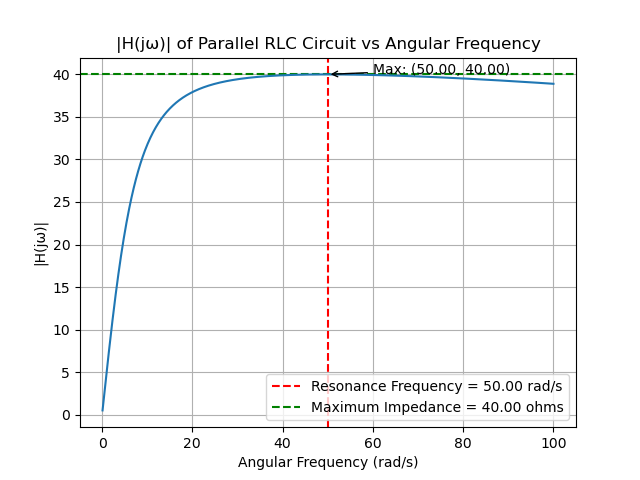
\includegraphics[width=1\linewidth]{ncert-physics/12/7/17/figs/m.png}
    \caption{Maximum impedance at resonating frequency in parallel RLC circuit}
\end{figure}

Hence it is proved that in parallel RLC circuit the total current is minimum at resonance frequency\\
   \text{(b)}\\
  At resonance frequency, Rms currents are\\
\begin{align}
\omega_0=\frac{1}{\sqrt{LC}}= 50rad/s\\
I_L=\frac{V}{\omega_0L}=\frac{230}{250}=0.92A\\
   I_C=\omega_0CV= 0.92 A\\
   I_R=\frac{V}{R}=\frac{230}{40}=5.75A
 \end{align}
